\documentclass[a4paper]{article}
% twocolumns
% \setlength{\columnsep}{1cm}

% principal packages
\usepackage{arxiv}          % styles package

% language packages
\usepackage[spanish]{babel} % spanish writing allowed
\selectlanguage{spanish}    % tildes allowed directly

% default template packages
\usepackage[utf8]{inputenc} % allow utf-8 input
\usepackage[T1]{fontenc}    % use 8-bit T1 fonts
\usepackage{hyperref}       % hyperlinks
\usepackage{url}            % simple URL typesetting
\usepackage{booktabs}       % professional-quality tables
\usepackage{amsfonts}       % blackboard math symbols
\usepackage{nicefrac}       % compact symbols for 1/2, etc.
\usepackage{microtype}      % microtypography
\usepackage{lipsum}         % lorem ipsum enabled
\usepackage{graphicx}       % support PDF, JPG, PNG, TIF files

% my packages
\usepackage{mathptmx}       % default font: Times New Roman
\usepackage{float}          % floating objects improvement
\usepackage{booktabs}       % professional-quality tables
\usepackage{verbatim}       % multi-line comments

% color links for to-do notes and hyper-ref
% \usepackage[colorinlistoftodos]{todonotes}
% \usepackage[colorlinks=true, allcolors=blue]{hyperref}

% page size and margins
% \usepackage[a4paper, top=2.5cm, bottom=2.5cm, left=2.5cm, right=2.5cm, marginparwidth=1.75cm]{geometry}

\graphicspath{ {./images/} }

% \pagenumbering{gobble}

% Bold: \textbf{text}
% Italics: \textit{text}

%%%%%%%%%%%%%%%%%%%%%%%%%%%%%%%%%%%%%%%%%%%%%%%%%%%%%%%%%%%%

% Document Body

%%%%%%%%%%%%%%%%%%%%%%%%%%%%%%%%%%%%%%%%%%%%%%%%%%%%%%%%%%%%

\title{\textbf{TP1 - Simulación de una Ruleta}}

\author{
    \textbf{Antonelli, Nicolás} \\
    Departamento de Ingeniería en Sistemas \\
    Universidad Tecnológica Nacional - FR Rosario \\
    Rosario, Zeballos 1341 \\
    \texttt{niconelli2@gmail.com} \\
  \And
    \textbf{Coauthor's Name} \\
    Departamento de Ingeniería en Sistemas \\
    Universidad Tecnológica Nacional - FR Rosario \\
    Rosario, Zeballos 1341 \\
    \texttt{coauthor@example.com} \\
    \small \date{}
}

\begin{document}
\maketitle
\begin{abstract}
La Simulación. Según R. E. Shannon: "La simulación es el proceso de diseñar un modelo de un sistema real y llevar a término experiencias con él, con la finalidad de comprender el comportamiento del sistema o evaluar nuevas estrategias -dentro de los límites impuestos por un cierto criterio o un conjunto de ellos - para el funcionamiento del sistema" \cite{simulacion_wiki}.

En este proyecto se ha realizado un análisis numérico y gráfico de los resultados obtenidos al simular una ruleta en Python, desde un punto de vista estadístico y haciendo uso de números pseudoaleatorios.
\end{abstract}

% keywords can be removed
%\keywords{First keyword \and Second keyword \and More}

\section{Introducción}
Este proyecto es el primer trabajo práctico de la cátedra "Simulación" (UTN FRRO, Departamento ISI). La idea fue que en esta simulación, donde lo que se modeliza es el funcionamiento de una ruleta 'europea'\cite{ruleta_wiki}, aparte de trabajar con números pseudoaleatorios para representar los números obtenidos al 'girarla' utilizamos listas (arrays) para hacer todo tipo de cálculos estadísticos tales como: la frecuencia relativa de un número en unas N tiradas de ruleta con respecto al total de números, el promedio (media estadística), varianza y desvío de una población conformada por los N números obtenidos, y como estos valores se comportan si vamos creciendo lentamente el N desde 0 hasta un valor dado en un input, como por ejemplo 'N = 500'. Todos estos valores fueron graficados para estudiarlos mejor. A su vez, se utilizaron matríces para poder calcular más de un juego de resultados de Ruleta a la vez, y graficar en simultáneo todo lo obtenido.


\section{Marco Teórico}
\label{sec:marco}
\subsection{Definiciones}
\label{sec:definiciones}
El valor de la frecuencia de aparición de un número X obtenido al azar en N tiradas de ruleta, es una \textit{Variable Aleatoria Discreta}, por la siguiente definición\cite{prob_est}:
\begin{quote}
''Una \textit{variable aleatoria} es una función que asigna a cada elemento del espacio muestral un número real. Una variable aleatoria es \textit{discreta} si su recorrido es un conjunto finito o infinito numerable (susceptible de ser contado)''. Lo anterior sucede es en este caso con un rango de (0, 1), calculado desde la cantidad de apariciones, dividido las N tiradas (N entero).
\end{quote}

Y también tenemos definida una población en cada momento que se realiza un cálculo: Las frecuencias de los 37 números que componen la Ruleta (del 0 al 36) obtenidas en N tiradas.

Ejemplo de parte de una población: \{0, 2, 3, 0...\} --> La primera parte de este Array equivale a que el número 0 salió 0 veces, el número 1 salió 2, el número 2 salió 3, el número 4 salió 0 veces... (y así hasta el 36).

\subsection{Fórmulas Empleadas}
\label{sec:formulas}

Cálculo de la Frecuencia Relativa de un Número X con respecto a los N números de la tirada. Dónde:
\begin{itemize}
    \item n es la frecuencia absoluta de un número, es decir, su cantidad de apariciones
    \item N es el tamaño de la población, es decir los N números obtenidos en la tirada.
    \item x es el número elejido a ser estudiado, cualquiera entre 0 y 36.
\end{itemize}

\begin{equation}
    \textit{f}_{x} = \frac {n_{x}} {\sum_{i=0}^{N}n_{i}}
    = \frac {n_{x}} {N}
\end{equation}

Cálculo de la Esperanza Matemática (en este caso es lo mísmo referirse a ella como Media o Promedio) de la Población. Dónde:
\begin{itemize}
    \item X es un número de la población
    \item \(\Re\) es el recorrido de la población (0, 36)
    \item \(P_{x}(X)\) es la probabilidad de ocurrencia de X
\end{itemize}
\begin{equation}
    \textit{E}(X) = \mu_{X} = \sum_{x \in \Re_{x}}X P_{x}(X)
\end{equation}

\begin{quote}
    Pero como  \(P_{x}(X)\) es lo mismo que hablar de \({f}_{x}\), entonces aplicando la fórmula (1) se puede sacar N (tamaño de la población) como factor común. De esta forma, solo multiplico dentro de la sumatoria, y divido una sola vez en el final, ahorrando tiempo de procesamiento. La fórmula entonces queda como la siguiente:
\end{quote}

\begin{equation}
    \textit{E}(X) = \mu_{X} = \frac { \sum_{x \in \Re_{x}}
    X n_{x} } { N }
\end{equation}

Cálculo de la Varianza de la Población. Dónde:
\begin{itemize}
    \item X es un número de la población
    \item \(\Re\) es el recorrido de la población (0, 36)
    \item \(P_{x}(X)\) es la probabilidad de ocurrencia de X
    \item \(\mu_{X}\) es la media de la población, calculada en (3)
\end{itemize}

\begin{equation}
    \textit{V}(X) = \sigma^2_{X} = \sum_{x \in \Re_{x}}
    (X - \mu_{X})^2 P_{x}(X)
\end{equation}

\begin{quote}
    Siguiendo el mismo razonamiento utilizado para a partir de la fórumla (2) sacar la fórumla (3), acá también se puede utilizar la fórmula (1) y sacar factor común N y ahorrar tiempo innecesario calculando divisiones demás en el código. La fórmula entonces queda como la siguiente:
\end{quote}

\begin{equation}
    \textit{V}(X) = \sigma^2_{X} = \frac { \sum_{x \in
    \Re_{x}} (X - \mu_{X})^2 X n_{x} } { N }
\end{equation}

Cálculo del Desvío de la Población. Dónde:
\begin{itemize}
    \item \(\sigma_{X}\) es la varianza de la población calculada en (5)
\end{itemize}

\begin{equation}
    \textit{D}(X) = \sigma_{X} = \sqrt{ \sigma^2_{X} }
\end{equation}


\section{Estrucura de la Simulación}
\label{sec:estructura}
Para componer este trabajo práctico, se ha utilizado íntegramente el lenguaje \textbf{Python}\cite{python_doc}, escrito el código en \textbf{Visual Studio Code}\cite{vs_code} con su correspondiente \textit{Plugin}. Para llegar al resultado final, se han probado y descartado varias librerías y módulos en el camino, que fueron reemplazadas por otras; tales como: la librería \textbf{statistics} que tenía funciones estadísticas fáciles de utilizar, pero ciertos límites en la cantidad de decimales a manejar con \textit{floats}, la librería \textbf{random} para números \textit{pseudoaleatorios}, pero se utilizó una mejor, entre otras. A continuación, se presenta lo que sí ha llegado hasta la \textit{versión final}:

\subsection{Metodología: Librerías y Módulos Utilizados}
\label{sec:metodologia}

\paragraph{Numpy}\cite{numpy_doc}
Esta librería tiene de todo. Primero, la utilización de \textit{Arrays y Matrices} en vez de \textit{Listas}, pues estas últimas son objetos, y con los arrays de Numpy se consigue una mayor eficiencia (es recomendable utilizar arrays y matrices de tamaño fijo, pues como no se almacena de forma contigua espacio extra con Numpy, tamaños variables destruyen esta eficiencia mayor pues aumentar el tamaño sería volver a construirlo).

Numpy Tiene un módulo llamado random (Numpy.Random) que se utilizó para conseguir los números pseudoaleatorios de una forma rápida, y si se necesita, se puede generar un Array de N longitud con todos valores aleatorios.
Numpy también posee fórmulas estadísticas muy potentes para calcular la \textit{media} (promedio), \textit{varianzas} y \textit{desvíos}.

Por último, también tiene un método llamado \textit{arange} que es como el \textit{for} de siempre, pero con algunos beneficios como que su \textit{Step} puede ser un float, o que se puede generar un array con él.

\paragraph{Pyplot}\cite{pyplot_doc}
Este módulo de la librería \textbf{matplotlib} es ideal para graficar toda la información calculada de una forma simple: unas pocas configuraciones y un array o lista a graficar. Su sintaxis es similar a usar \textbf{Matlab}. Los gráficos que genera son muy personalizables y rápidos de generarse. También posee la posibilidad de hacer \textit{Subplots}, es decir más de una gráfica en simultáneo, y plottearlas a todas juntas en una misma ventana.

\subsection{Método de Resolución Aplicado}
\label{sec:resolución}

Para hacerlo breve, ya que el código de la simulación tiene comentarios paso-a-paso explicando como funciona, la idea es la siguiente:
\paragraph{Primero} se pide un número N de tiradas de ruleta, y un número X a estudiar su frecuencia.
\paragraph{Segundo} se calculan los valores esperados (Frecuencia Relativa de X, y valores de la población: media, variación y desvío.
\paragraph{Tercero} se generan cuatro matríces, una para cada parámetro a estudiar, de tamaño (6xN), que se puede pensar como 6 arrays de tamaño N, uno para cada \textit{Conjunto de Resultados}. \textbf{¿Porqué calcular más de un Array de resultados?} Pues porque primero se pide graficar uno solo, pero luego se pide graficar en simultáneo entre 5 y 10 resultados.
\paragraph{Cuarto} se llena para cada uno de los 4 parámetro a estudiar, cada uno de los 6 array de resultados, cargando en un for o un arange anidado a otro for o arange: los valores que te da el aplicar la fórmula del parámetro correspondiente a una población de números aleatorios no-fija, ya que arranca en 0 (1era posición del array) y en cada loop va calculando con 1 tirada más que la anterior, hasta la última iteración donde calcula los parámetros con respecto a una población N (última población del array).
\paragraph{Quinto} se toman las posiciones [0] de cada matriz, osea el conjunto de resultados 0: Un array lleno de frecuencias relativas, uno lleno de promedios (medias), otro de varianzas y otro de desvíos. Se plottean los 4 gráficos (stack de 4 subplots) de ese conjunto de resultados en una misma ventana. Luego, se grafican los 6 conjuntos de resultados con un color cada uno, de la misma forma que lo anterior, solo que todos en simultáneo.

\newpage
\section{Gráficas Obtenidas}
\label{sec:graficas}

\subsection{Etiquetas de las Gráficas}
\label{sec:etiquetas}

\begin{itemize}
    \item \textbf{FRE}: Frecuencia Relativa Esperada
    \item \textbf{FRN}: Frecuencia Relativa de un número X con respecto a las N Tiradas
    \item \textbf{VPE}: Valor Promedio Esperado
    \item \textbf{VPN}: Valor Promedio con respecto a las N Tiradas
    \item \textbf{VVE}: Valor de la Varianza Esperado
    \item \textbf{VVN}: Valor de la Varianza con respecto a las N Tiradas
    \item \textbf{VDE}: Valor del Desvío Esperado
    \item \textbf{VDN}: Valor del Desvío con respecto a las N Tiradas
\end{itemize}

\subsection{Población Pequeña}
\label{sec:pobpeq}

Gráficas obtenidas con el estudio de una población pequeña. Rango de N = (0, 20). Primero gráfica de un solo conjunto resolución, luego de los 6 en simultáneo.

\begin{figure}[H]
    \centering
    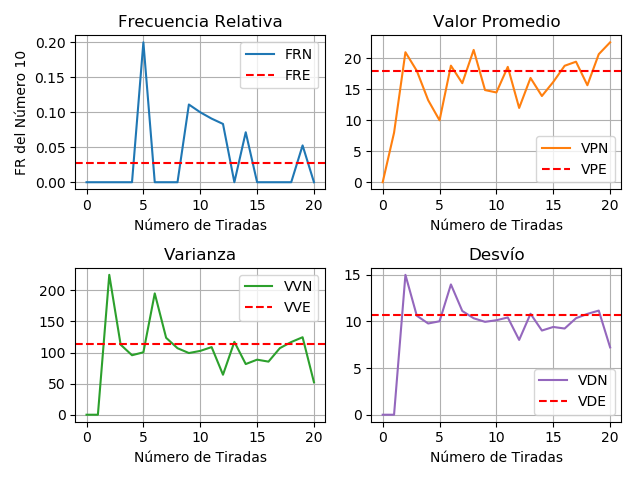
\includegraphics[width=0.75\textwidth]{./graphs/graph_iterations_20.png}
    \caption{\label{fig:img1}Un conjunto de Resolución. De 0 a 20 Tiradas.}
\end{figure}

\begin{figure}[H]
    \centering
    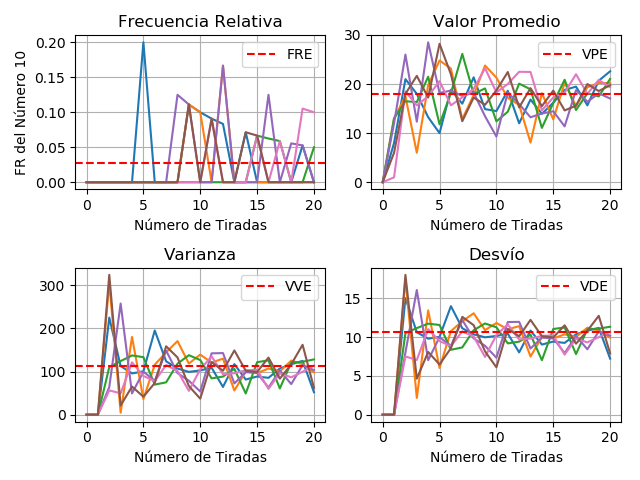
\includegraphics[width=0.75\textwidth]{./graphs/multi_graph_iterations_20.png}
    \caption{\label{fig:img2}Los 6 conjuntos de Resolución en simultáneo. De 0 a 20 Tiradas.}
\end{figure}

\subsection{Población Mediana}
\label{sec:pobmed}

Gráficas obtenidas con el estudio de una población mediana. Rango de N = (0, 120). Primero gráfica de un solo conjunto resolución, luego de los 6 en simultáneo.

\begin{figure}[H]
    \centering
    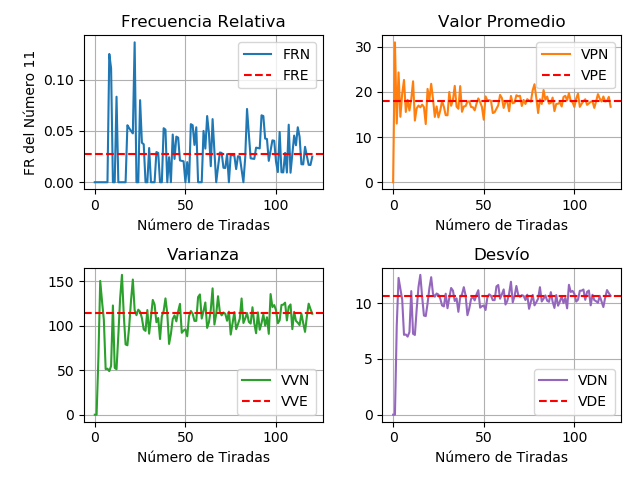
\includegraphics[width=0.75\textwidth]{./graphs/graph_iterations_120.png}
    \caption{\label{fig:img3}Un conjunto de Resolución. De 0 a 120 Tiradas.}
\end{figure}

\begin{figure}[H]
    \centering
    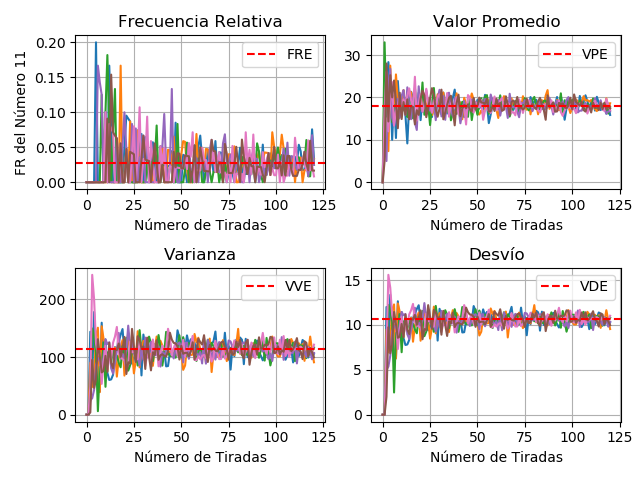
\includegraphics[width=0.75\textwidth]{./graphs/multi_graph_iterations_120.png}
    \caption{\label{fig:img4}Los 6 conjuntos de Resolución en simultáneo. De 0 a 120 Tiradas.}
\end{figure}

\subsection{Población Grande}
\label{sec:pobgra}

Gráficas obtenidas con el estudio de una población grande. Rango de N = (0, 1000). Primero gráfica de un solo conjunto resolución, luego de los 6 en simultáneo.

\begin{figure}[H]
    \centering
    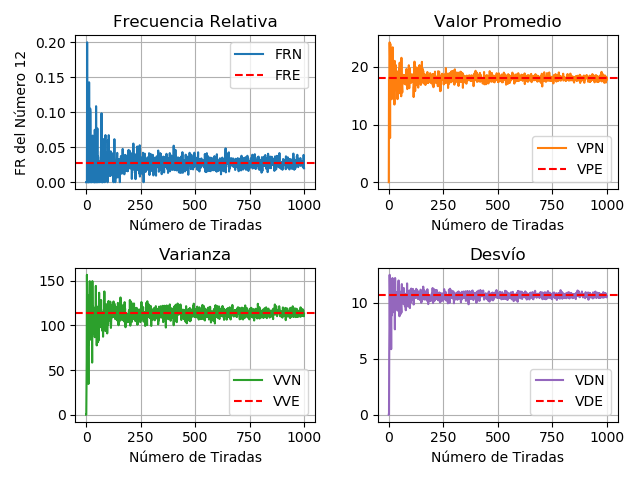
\includegraphics[width=0.75\textwidth]{./graphs/graph_iterations_1000.png}
    \caption{\label{fig:img5}Un conjunto de Resolución. De 0 a 1000 Tiradas.}
\end{figure}

\begin{figure}[H]
    \centering
    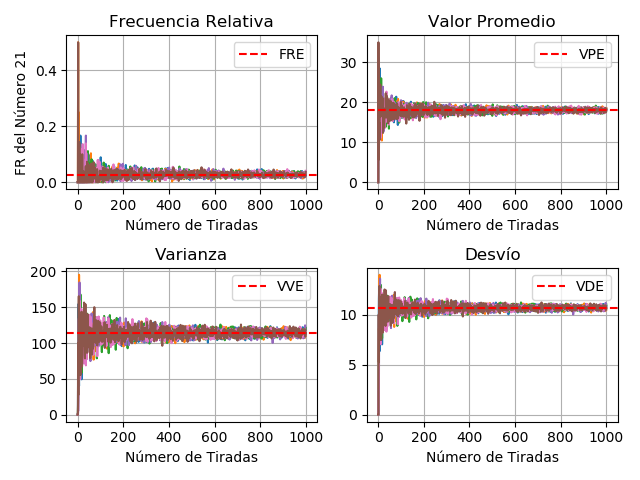
\includegraphics[width=0.75\textwidth]{./graphs/multi_graph_iterations_1000.png}
    \caption{\label{fig:img6}Los 6 conjuntos de Resolución en simultáneo. De 0 a 1000 Tiradas.}
\end{figure}


\section{Conclusiones}
\label{sec:conclusiones}
Luego de analizar el comportamiento de los conjuntos de resultados en las gráficas, se aprecia que en un N pequeño los valores obtenidos están bastante alejados de los valores esperados. Sin embargo, aumentando N, estos valores van "convergiendo" lentamente a un rango de valores muy próximo a los valroes esperados. La forma gráfica del acotamiento de estos valores conforme aumenta N recuerda a el movimiento armónico amortiguado.
\bigskip
\newline
Podemos concluir entonces que si N tiende a \(\infty\), todos los valores obtenidos serán aproximadamente iguales a los valores esperados.
\bigskip
\newline
Otra observación interesante es que si en las gráficas donde aparecen en simultáneo varios conjuntos de resultados tomamos los valores de cada una y (sin realizar cálculos, a simple vista) podemos ver que los promedios de los mismos, aún a pesar de lo errático q son en poblaciones pequeñas, son bastante más próximos a los valores esperados.


\newpage
\bibliographystyle{unsrt}  
\begin{thebibliography}{1}

\bibitem{simulacion_wiki}
    Wikipedia ES.
    \newblock Definición de Simulación. \\
    \newblock \underline{\url{https://es.wikipedia.org/wiki/Simulación}}

\bibitem{ruleta_wiki}
    Wikipedia ES.
    \newblock Definición de Ruleta. \\
    \newblock \underline{\url{https://es.wikipedia.org/wiki/Ruleta}}

\bibitem{prob_est}
    Raúl Katz - Pablo Sabatinelli (2018).
    \newblock Probabilidad y Estadística: Variables Aleatorias Discretas y algunas Distribuciones de Probabilidad

\bibitem{python_doc}
    Python Doc.
    \newblock Python 3.8.2 | Documentación Oficial. \\
    \newblock \underline{\url{https://docs.python.org/3/}}

\bibitem{vs_code}
    Microsoft (VSC).
    \newblock Visual Studio Code Official Webpage \\
    \newblock \underline{\url{https://code.visualstudio.com/}}

\bibitem{numpy_doc}
    Numpy Doc.
    \newblock Numpy 1.18 | Documentación Oficial. \\
    \newblock \underline{\url{https://numpy.org/doc/1.18/}}

\bibitem{pyplot_doc}
    Pyplot Doc.
    \newblock Pyplot 3.1.1 | Documentación Oficial. \\
    \newblock \underline{\url{https://matplotlib.org/3.1.1/api/\_as\_gen/matplotlib.pyplot.html}}

\end{thebibliography}


\end{document}
